\chapter{Problemi NL-completi} \label{ch:capitolo17}
\subsection{Il grafo delle computazioni}
Data una macchina di Turing M, un input w e un intero $K >= s_M(n)$, costruiamo il grafo G(M, w) con
\begin{itemize}
    \item I vertici di G(M, w) sono le configurazioni istantanee di M con input w e spazio $<=$ K sul nastro di lavoro, oltre a un ulteriore vertice t(M, w)
    \item Le frecce sono le coppie (C, C') tali che C $\vdash$M C' e, inoltre, le coppie (C,t(M, w)) con C $\vdash /$M
\end{itemize}
\textbf{Osservazione}\\
G(M, w) ha n $2^{O(K)}$ vertici e $n^2$ $2^{O(K)}$ frecce.\\\\
\textbf{Applicazione}\\
\begin{center}
    $c_M(n) = n · 2^{O(s_M(n))}$
\end{center}
Invero, una computazione che accetta w corrisponde a un cammino in G(M, w) dalla configurazione iniziale fino a t(M, w).
Se priva di cicli, la sua lunghezza è minore del numero dei vertici.
\subsection{Un'applicazione}
\textbf{Proposizione}\\
\begin{center}
    NL $\subseteq$ P.
\end{center}
\textbf{Dimostrazione}\\
Sia S $\in$ NL e sia M una macchina di Turing non deterministica che accetta S con
\begin{center}
    $s_M(n) <= c \log2(n)$
\end{center}
Per decidere S si può usare la seguente procedura deterministica su input w
\begin{enumerate}
    \item costruire G(M, w), con $K = |c \log2(n)|$
    \item cercare un cammino dalla configurazione iniziale a t(M, w)
    \item se tale cammino esiste, accettare, altrimenti rifiutare.
\end{enumerate}
Il numero dei vertici di G(M, w) è $n · 2^{O(\log2(n))} = n^{O(1)}$, e ognuno di essi è descritto da O(log n) bit.
\\Pertanto la procedura descritta è in P.
\subsection{L=NL?}
\textbf{Definizione}\\
Siano S, S' due problemi su alfabeti finiti A, A' rispettivamente.
\\Scriviamo
\begin{center}
    $S <=_{\log} S'$
\end{center}
se esiste una funzione totale $f : A^* \mapsto A'^*$, computabile deterministicamente in spazio logaritmico, tale che per ogni w $\exists$ A*
\begin{center}
    w $\in$ S $\Longleftrightarrow$ f(w) $\in$ S'
\end{center}
\textbf{Osservazione}\\
Non è evidente che la relazione $<=$ log sia un pre-ordine.
\\In effetti, non è banale trovare un algoritmo che calcoli in spazio
polinomiale la composizione di due funzioni calcolabili in spazio polinomiale.
\subsection{Riduzioni in spazio logaritmico}
Data una funzione $f : A^* \mapsto A'^*$ denotiamo con $\hat{f}$ la funzione di $A^*$ x N in A' definita da
\begin{itemize}
    \item $\hat{f}$(w, n)=n-esima lettera di f(w)
\end{itemize}
\textbf{Lemma}\\
La funzione f si può calcolare in spazio logaritmico se e solo se $\hat{f}$ si può calcolare in spazio logaritmico
\subsection{Dimostrazione}
Supponiamo che f sia calcolata da una macchina di Turing deterministica M in spazio logaritmico.
Ovviamente, M avrà un nastro di output write-only. La funzione $\hat{f}$ è calcolata da una macchina di Turing M' ottenuta
modificando M nel modo seguente:
\begin{itemize}
    \item aggiungiamo sul nastro di lavoro un contatore, con valore iniziale 1
    \item le istruzioni di spostamento della testina sul nastro di output sono sostituite da incrementi/decrementi del contatore
    \item si esegue l’istruzione di scrittura sul nastro di output solo se il valore del contatore è n
\end{itemize}
Lo spazio per il contatore è $\log2$ l(f(w)).
\\Poichè NL $\subseteq$ P, si ha $\log2$
l(f (w)) $=$ O($\log2$ l(w))
\subsection{La relazione $<=\log$}
\textbf{Proposizione}\\
Siano S, S', S'' problemi definiti su alfabeti finiti A, A', A'' rispettivamente.
\begin{itemize}
    \item Se S $<=_{\log}$ S' e S' $<=_{\log}$ S'', allora S $<=_{\log}$  S''
    \item Se S $<=_{\log}$ S' e S $\in$L, allora S $\in$ L.
    \item Se S $<=_{\log}$ S' e S' $\in$ NL, allora S $\in$ NL.
\end{itemize}
\textbf{Dimostrazione}\\
Siano f e g, rispettivamente, le riduzioni di S a S' e di S' a S'' calcolabili in spazio logaritmico.
\\Denotiamo con M la macchina di Turing che calcola $\hat{f}$ se con M' la macchina di Turing che calcola g.
Costruiamo una macchina di Turing M'' che calcola f ° g, simulando simultaneamente M e M'
\subsection{Dimostrazione}
\begin{itemize}
    \item Sul nastro di input scriviamo la parola w su cui calcolare f ° g
    \item Sul nastro di lavoro registriamo
        \begin{itemize}
            \item il contenuto del nastro di lavoro della macchina M'
            \item la posizione della testina di lettura sul nastro di input di M'
            \item una parte del nastro è riservato alla simulazione di M
        \end{itemize}
    \item La computazione funziona nel modo seguente
    \begin{itemize}
        \item si legge la posizione n della testina del nastro di input di M'
        \item  si calcola f (w, n) usando il nastro di input e la parte riservata sul nastro di lavoro
        \item  si simula un passo della computazione di M' utilizzando l’input f (w, n) e il nastro di lavoro e si aggiorna il valore di n
    \end{itemize}
    \item lo spazio necessario è logaritmico
\end{itemize}
Le altre due dimostrazioni sono analoghe.
\newpage
\subsection{NL-completezza}
\textbf{Definizione}\\
Un problema T si dice NL-arduo se per ogni S $\in$ NL si ha S $<=_{\log}$ T.\\
Un problema T si dice NL-completo se sta in NL ed è NL-arduo.\\\\
\textbf{Osservazione}\\
Sia T un problema NL-completo.\\
Allora si ha T $\in$ L se e soltanto se L $=$ NL
\subsection{Gap}
\textbf{Problema di accessibilità nei grafi}\\
\textbf{Input:} Un grafo diretto G $=$ (V, E) e due vertici $t_0,t_1 \in V$\\
\textbf{Output:} SI se in G c’è un cammino da $t_0$ a $t_1$, NO altrimenti.\\\\
\textbf{Teorema}\\
GAP è un problema NL-completo.\\\\
\textbf{Dimostrazione}\\
\begin{center}
    GAP $\in$ NL
\end{center}
Una procedura non deterministica che accetta GAP in spazio logaritmico è
la seguente.
\begin{figure}[htp]
    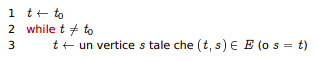
\includegraphics[scale=0.9]{tesi_stile/img/foto1cap17.png}
\end{figure}
\newpage
\subsection{GAP è NL-arduo}
Sia S $\in$ NL.
\\Dobbiamo trovare una riduzione di S a GAP, calcolabile in spazio logaritmico.
\\Sia M una macchina di Turing non deterministica che accetta S in spazio
logaritmico.
\\A ogni input w del problema S associamo la tripla
\begin{center}
    $f (w) = (G(M, w),t_0,t(M, w))$ ove
\end{center}
\begin{itemize}
    \item G(M, w) è il grafo delle computazioni di M su w
    \item $t_0$ è la configurazione iniziale
\end{itemize}
È facile verificare che f è una riduzione di S a GAP.
\\Un’analisi attenta mostra che f si può calcolare in spazio logaritmico.


